\subsection{Quantum Circuits}

This section aims to show that it is possible to change digital computing into something that is compatible with quantum computers.

\subsubsection{Digital logic}

Every digital computing operation can be built up from NAND logic gates \cite{sheffer1913set}

\begin{figure}[h]
  \centering
  \begin{subfigure}[h]{0.4\textwidth}
    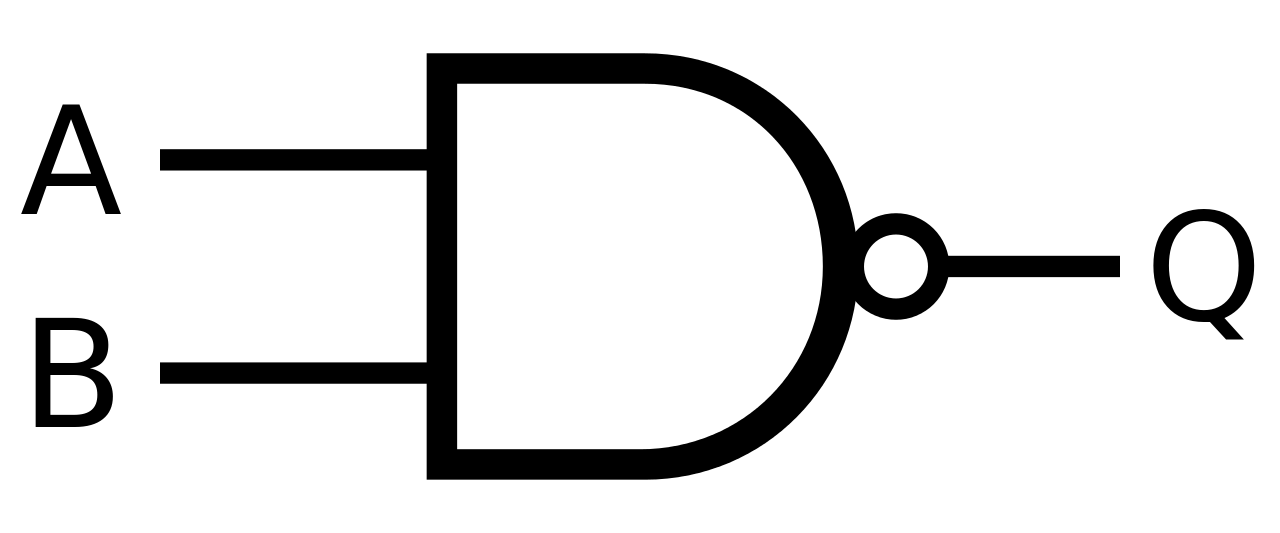
\includegraphics[width=0.7\textwidth]{NAND_ANSI_Labelled_svg.png}
    \caption{The NAND logic gate \cite{nandwiki}.}
    \label{fig:NAND}
  \end{subfigure}
~
  \begin{subfigure}[h]{0.4\textwidth}
    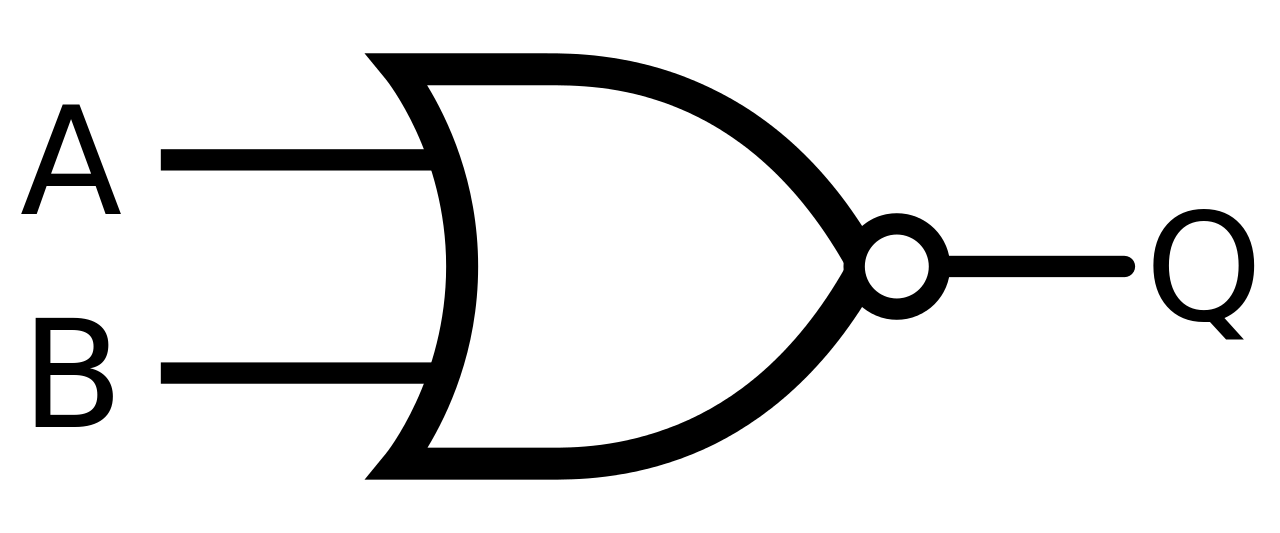
\includegraphics[width=0.7\textwidth]{NOR_ANSI_Labelled_svg.png}
    \caption{The NOR logic gate \cite{norwiki}.}
    \label{fig:NOR}
    \end{subfigure}
\end{figure}

reversible logic

%%%%%%%%% circuit 1 
\begin{figure}[h!]
\begin{align*}
\Qcircuit @C=0.5cm @R=0.7cm{
%1
&\lstick{S_1} &\gate{H} &\ctrl{1} &\qw \\
%0
&\lstick{S_0} &\ctrl{-1} &\targ &\qw \\
}
\end{align*}
\caption{Schur transform for 2 qubits}
\label{cir:vanilla2}
\end{figure}

